\tikzset{every picture/.style={line width=0.75pt}} %set default line width to 0.75pt        

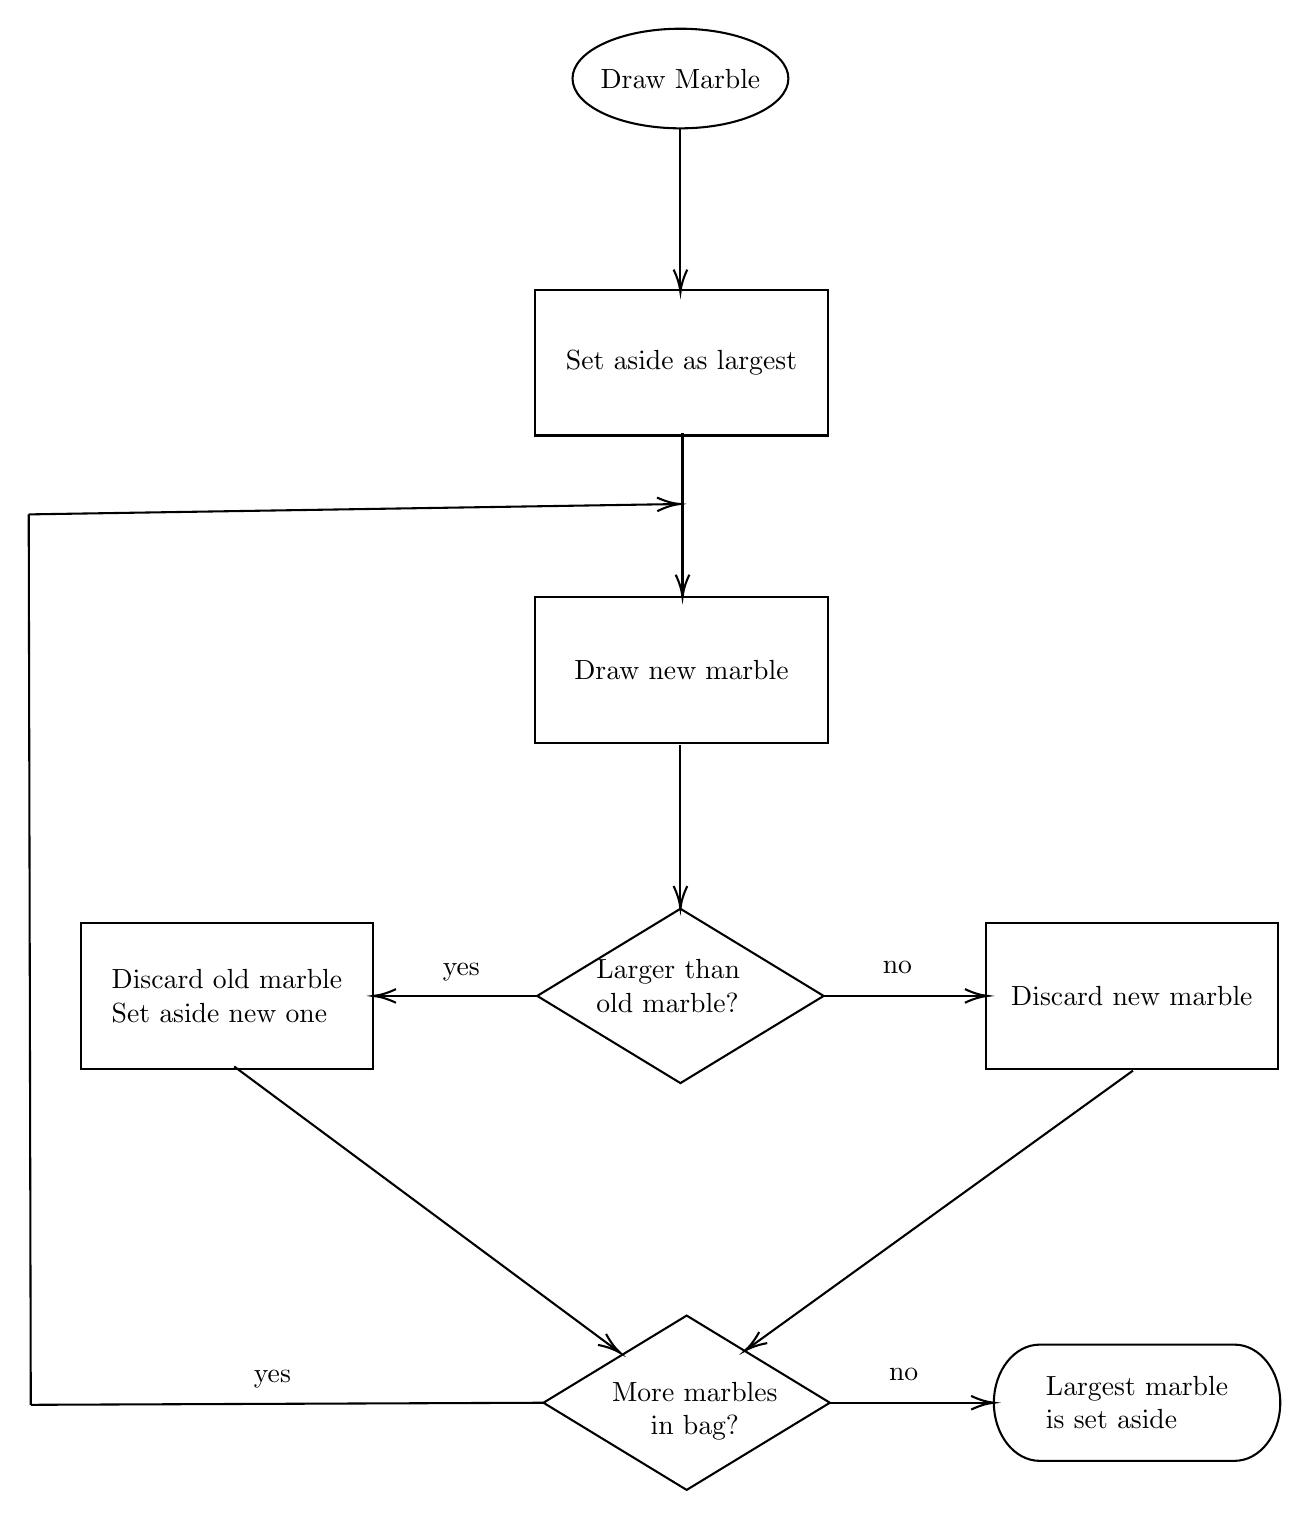
\begin{tikzpicture}[x=0.75pt,y=0.75pt,yscale=-1,xscale=1]
%uncomment if require: \path (0,812); %set diagram left start at 0, and has height of 812

%Shape: Ellipse [id:dp7078776640454232] 
\draw   (270,32) .. controls (270,18.75) and (293.28,8) .. (322,8) .. controls (350.72,8) and (374,18.75) .. (374,32) .. controls (374,45.25) and (350.72,56) .. (322,56) .. controls (293.28,56) and (270,45.25) .. (270,32) -- cycle ;
%Shape: Boxed Line [id:dp972704207942342] 
\draw    (322,56) -- (322,133) ;
\draw [shift={(322,135)}, rotate = 270] [color={rgb, 255:red, 0; green, 0; blue, 0 }  ][line width=0.75]    (10.93,-3.29) .. controls (6.95,-1.4) and (3.31,-0.3) .. (0,0) .. controls (3.31,0.3) and (6.95,1.4) .. (10.93,3.29)   ;
%Flowchart: Process [id:dp12474322255758397] 
\draw   (252,134) -- (393,134) -- (393,204) -- (252,204) -- cycle ;
%Shape: Boxed Line [id:dp03382264465030782] 
\draw    (8,242) -- (319.71,237.03) ;
\draw [shift={(321.71,237)}, rotate = 179.09] [color={rgb, 255:red, 0; green, 0; blue, 0 }  ][line width=0.75]    (10.93,-3.29) .. controls (6.95,-1.4) and (3.31,-0.3) .. (0,0) .. controls (3.31,0.3) and (6.95,1.4) .. (10.93,3.29)   ;
%Shape: Boxed Line [id:dp28644614408481495] 
\draw    (323,203) -- (323,280) ;
\draw [shift={(323,282)}, rotate = 270] [color={rgb, 255:red, 0; green, 0; blue, 0 }  ][line width=0.75]    (10.93,-3.29) .. controls (6.95,-1.4) and (3.31,-0.3) .. (0,0) .. controls (3.31,0.3) and (6.95,1.4) .. (10.93,3.29)   ;
%Flowchart: Process [id:dp9898963336751274] 
\draw   (252,282) -- (393,282) -- (393,352) -- (252,352) -- cycle ;
%Flowchart: Decision [id:dp6216008434832396] 
\draw   (322,432) -- (391,474) -- (322,516) -- (253,474) -- cycle ;
%Shape: Boxed Line [id:dp7931040026577363] 
\draw    (322,353) -- (322,430) ;
\draw [shift={(322,432)}, rotate = 270] [color={rgb, 255:red, 0; green, 0; blue, 0 }  ][line width=0.75]    (10.93,-3.29) .. controls (6.95,-1.4) and (3.31,-0.3) .. (0,0) .. controls (3.31,0.3) and (6.95,1.4) .. (10.93,3.29)   ;
%Shape: Boxed Line [id:dp6715019356060254] 
\draw    (253,474) -- (176,474) ;
\draw [shift={(174,474)}, rotate = 360] [color={rgb, 255:red, 0; green, 0; blue, 0 }  ][line width=0.75]    (10.93,-3.29) .. controls (6.95,-1.4) and (3.31,-0.3) .. (0,0) .. controls (3.31,0.3) and (6.95,1.4) .. (10.93,3.29)   ;
%Shape: Boxed Line [id:dp45065332069120023] 
\draw    (391,474) -- (468,474) ;
\draw [shift={(470,474)}, rotate = 180] [color={rgb, 255:red, 0; green, 0; blue, 0 }  ][line width=0.75]    (10.93,-3.29) .. controls (6.95,-1.4) and (3.31,-0.3) .. (0,0) .. controls (3.31,0.3) and (6.95,1.4) .. (10.93,3.29)   ;
%Flowchart: Process [id:dp8374841194029297] 
\draw   (469,439) -- (610,439) -- (610,509) -- (469,509) -- cycle ;
%Flowchart: Process [id:dp16793270470552768] 
\draw   (33,439) -- (174,439) -- (174,509) -- (33,509) -- cycle ;
%Flowchart: Decision [id:dp8898317341435751] 
\draw   (325,628) -- (394,670) -- (325,712) -- (256,670) -- cycle ;
%Straight Lines [id:da18982359592399445] 
\draw    (540,510) -- (354.62,643.83) ;
\draw [shift={(353,645)}, rotate = 324.17] [color={rgb, 255:red, 0; green, 0; blue, 0 }  ][line width=0.75]    (10.93,-3.29) .. controls (6.95,-1.4) and (3.31,-0.3) .. (0,0) .. controls (3.31,0.3) and (6.95,1.4) .. (10.93,3.29)   ;
%Shape: Boxed Line [id:dp7328385757826796] 
\draw    (107,508) -- (291.39,644.81) ;
\draw [shift={(293,646)}, rotate = 216.57] [color={rgb, 255:red, 0; green, 0; blue, 0 }  ][line width=0.75]    (10.93,-3.29) .. controls (6.95,-1.4) and (3.31,-0.3) .. (0,0) .. controls (3.31,0.3) and (6.95,1.4) .. (10.93,3.29)   ;
%Shape: Boxed Line [id:dp04108068314750124] 
\draw    (394,670) -- (471,670) ;
\draw [shift={(473,670)}, rotate = 180] [color={rgb, 255:red, 0; green, 0; blue, 0 }  ][line width=0.75]    (10.93,-3.29) .. controls (6.95,-1.4) and (3.31,-0.3) .. (0,0) .. controls (3.31,0.3) and (6.95,1.4) .. (10.93,3.29)   ;
%Shape: Boxed Line [id:dp2583793005729782] 
\draw    (256,670) -- (9,671) ;
%Shape: Boxed Line [id:dp07004372573074047] 
\draw    (8,242) -- (9,671) ;
%Flowchart: Terminator [id:dp5241120411854552] 
\draw   (495.08,642) -- (588.92,642) .. controls (601.11,642) and (611,654.54) .. (611,670) .. controls (611,685.46) and (601.11,698) .. (588.92,698) -- (495.08,698) .. controls (482.89,698) and (473,685.46) .. (473,670) .. controls (473,654.54) and (482.89,642) .. (495.08,642) -- cycle ;

% Text Node
\draw (322,32) node   [align=left] {Draw Marble};
% Text Node
\draw (322.5,169) node   [align=left] {Set aside as largest};
% Text Node
\draw (322.5,317) node   [align=left] {Draw new marble};
% Text Node
\draw (280,455) node [anchor=north west][inner sep=0.75pt]   [align=left] {Larger than\\ old marble?};
% Text Node
\draw (206,462.5) node [anchor=west] [inner sep=0.75pt]   [align=left] {yes};
% Text Node
\draw (418,456) node [anchor=north west][inner sep=0.75pt]   [align=left] {no};
% Text Node
\draw (539.5,474) node   [align=left] {Discard new marble};
% Text Node
\draw (103.5,474) node   [align=left] {Discard old marble\\Set aside new one};
% Text Node
\draw (328.93,674) node   [align=left] {\begin{minipage}[lt]{67.9pt}\setlength\topsep{0pt}
\begin{center}
More marbles \\in bag?
\end{center}

\end{minipage}};
% Text Node
\draw (115,658.5) node [anchor=west] [inner sep=0.75pt]   [align=left] {yes};
% Text Node
\draw (421,652) node [anchor=north west][inner sep=0.75pt]   [align=left] {no};
% Text Node
\draw (542,670) node   [align=left] {Largest marble\\is set aside};


\end{tikzpicture}
